\chapter{Encaminamiento con GeoPackage}
\label{ch:geopackage_routing}

\begin{chapsummary}
	De partida, se presenta una explicación de qué datos son necesarios y cómo obtenerlos. Luego se explican algunas técnicas de manipulación para filtrar los datos que consideremos interesantes en el estudio. Después de esto, se presenta la estructura que esta topología tomará en el contenedor de datos. A continuación, se detalla el procedimiento a seguir para obtener dicha topología a partir de los datos filtrados. Finalmente, se demuestra las posibilidades de encaminamiento con dicho contenedor de datos.
\end{chapsummary}

\section*{Introducción}
Este capítulo es el principal del desarrollo y está dedicado a analizar la viabilidad de generar y estructurar una topología de alguna red geográfica, como puedan ser carreteras o ferroviaria, y su almacenamiento en un contenedor GeoPackage. Esto se enlaza con la presencia de un caso práctico en el que se genera la topología de red del término municipal de Granada, partiendo de unos datos generales sin tratar, hasta conseguir un contenedor \textit{GeoPackage} donde se encuentre la información relevante, así como la misma topología de red.

Se pretende llevar un desarrollo mixto, ligando un análisis general con el caso práctico, explicando qué hacer en ámbitos generales y después aplicar lo explica al ámbito concreto de la ciudad de Granada. Concretamente, para el caso práctico, además se nombran bastantes herramientas usadas y cómo se integran con aquellas desarrolladas.

\section{Obtención de los Datos}
	El pilar básico de cualquier análisis es la información, como conjunto de datos estructurado. En el caso del objeto de este estudio, necesitamos datos que nos proporcione información sobre una red de carreteras sobre las que queramos aplicar técnicas de encaminamiento, de búsquedas de caminos. A grandes rasgos, existen dos posibilidades. 
	
	Por una parte, podemos generar la información geográfica a partir de la digitalización \autocite[140-152]{bolstad}. Esto es, por ejemplo, mediante el uso de ortofotografías (fotografías corregidas a un ángulo ortogonal a la tierra) podemos generar un mapa vectorial, sea manual o pseudoautomatizado, pero este es un proceso costoso. 
	
	Por suerte, también existe la posibilidad de usar datos recopilados por otras fuentes, ya sean puestos a libre disposición o como producto a vender. Estas pueden ser distribuidas por algún proyecto gubernamental, empresarial o comunitario, e incluso por particulares.
	
	En definitiva, los datos de partida, irrelevante sea su origen, deben contener, al menos, suficiente información sobre una estructura en red sobre la que podamos extraer una topología válida, por ejemplo, una red de carreteras de un municipio o la red ferroviaria de un país.
	
	\subsection*{Caso Práctico}
	Se parte de los datos geográficos de toda España\autocite*{GeofabrikSpa}, recopilados por el proyecto \textit{OpenStreetMap} y empaquetados de forma gratuita por la empresa \textit{GeoFabrik}, con un formato \texttt{XML} comprimido en \texttt{ProtoBuf}\footnote{Protocol Buffers: Protocolo de serialización diseñado por Google. \url{https://developers.google.com/protocol-buffers/}}.
	
	\begin{figure}[htbp]
		\centering
		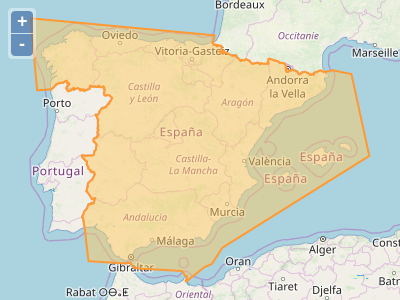
\includegraphics[width=0.45\textwidth]{img/source_data.png}
		\caption[Extensión de los datos originales]{Los datos comprenden la extensión vista en la figura, siendo gran parte de la península ibérica y las islas de Majorca, y no solo contienen información de carreteras, si no también términos municipales, reservas naturales, edificios, entre muchas otras cosas.}
	\end{figure}
	
	Estos datos contienen, en términos de \textit{OpenStreetMap}, elementos \textsc{Node}, \textsc{Way} y \textsc{Relation}. Para un estudio básico, basta con las primitivas \textsc{Way}, que forman las líneas que describen la composición geográfica de los camino, así como atributos que nos permitan seleccionar qué datos nos interesan. Concretamente, usaremos el atributo \texttt{highway} para identificar qué tipo de carretera representa y eliminar aquellos que no tengan relevancia.

\section{Transformaciones y Filtrado}
	
%	\subsection*{Reducción espacial}
	Muy comúnmente, es de interés profundizar en un área concreta para realizar análisis con un ámbito más específico del que nos proporcionan los datos originales. Cuando esto ocurre, es conveniente utilizar operaciones espaciales, como recorte (o \textit{clipping} \autocite[354--355]{bolstad}), delimitando el área a conservar con un polígono. 
	
	\begin{figure}[htbp]
		\begin{subfigure}{0.5\textwidth}
			\centering
			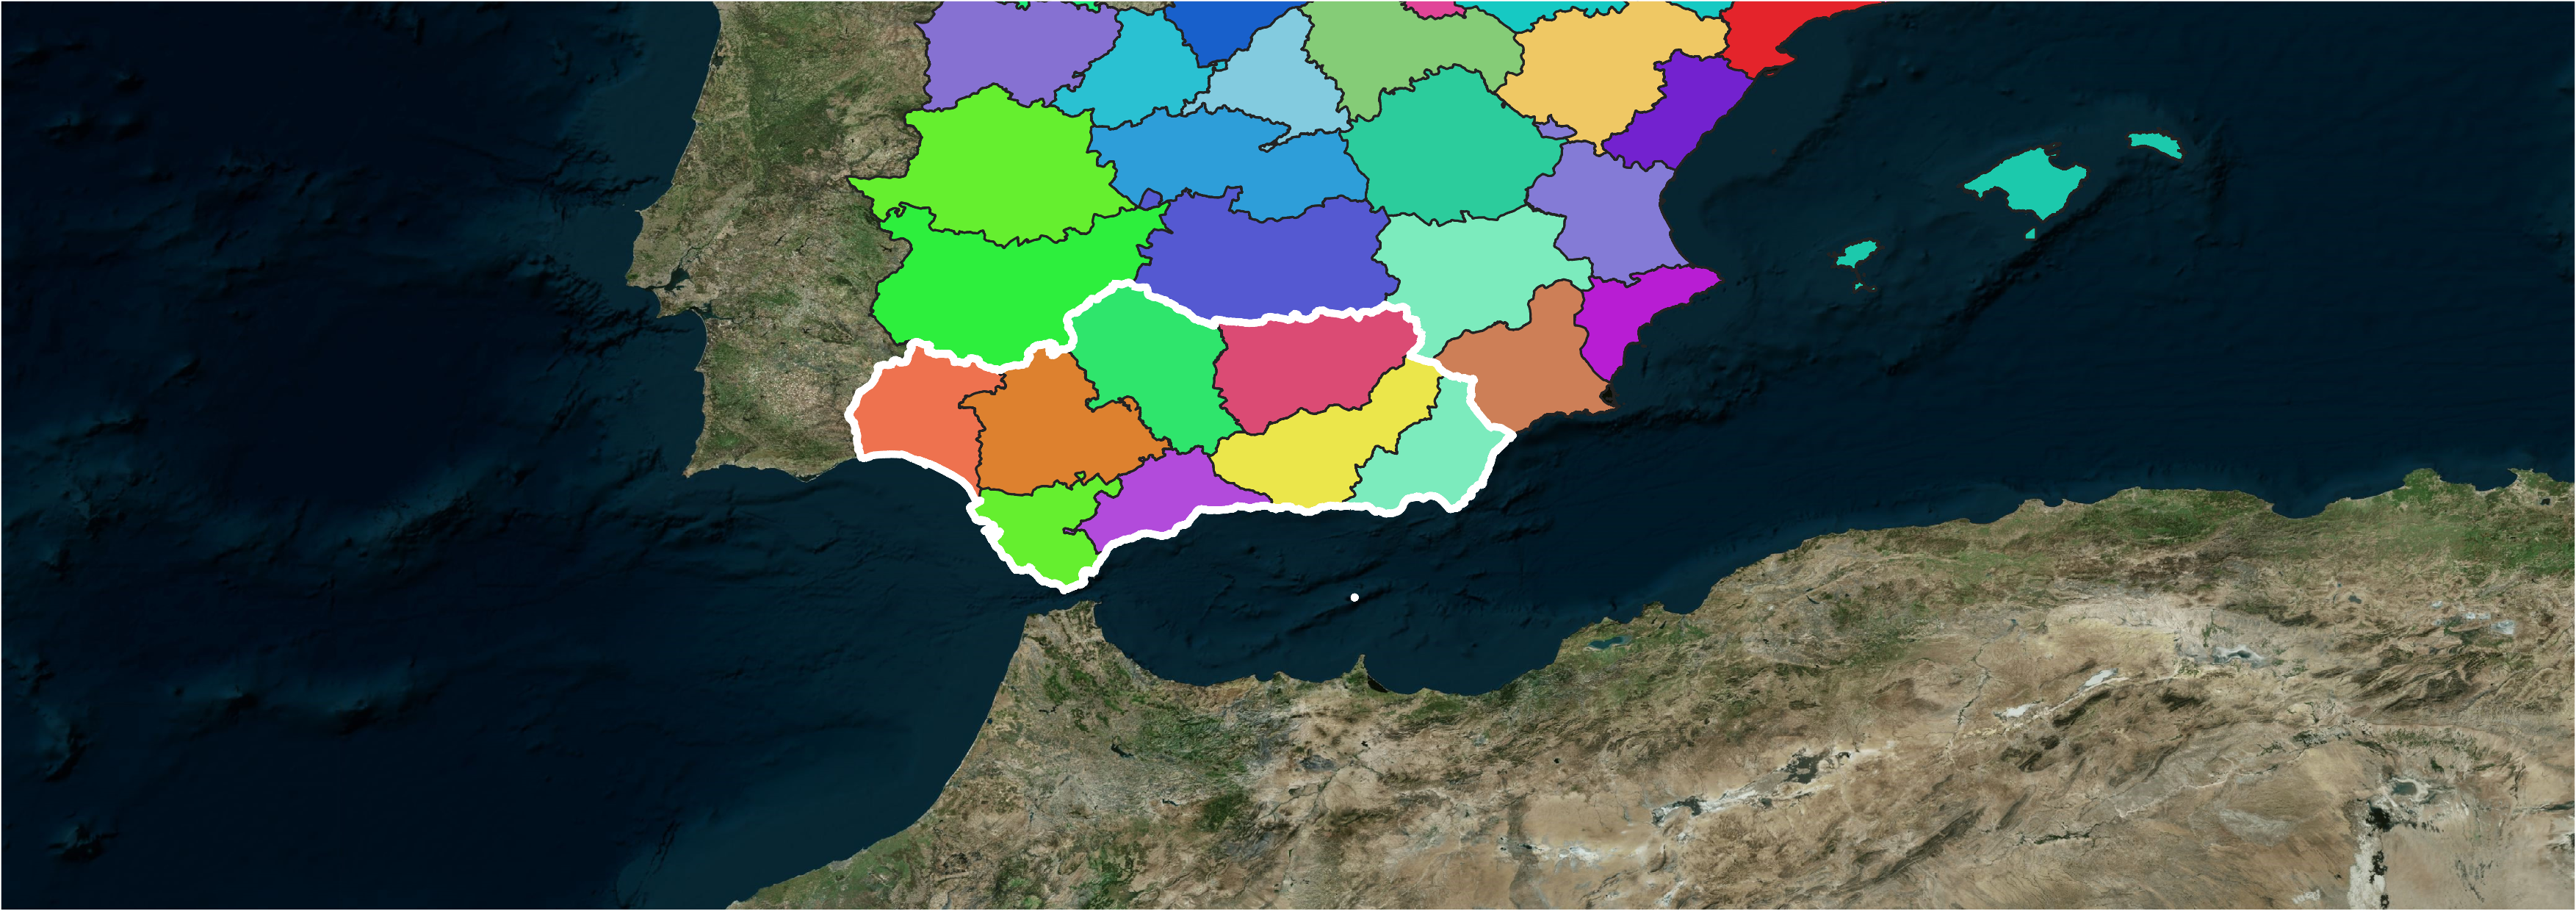
\includegraphics[width=.95\textwidth]{img/provinces_clip_before.png}
			\subcaption{\textit{Antes:} Provincias de España}
		\end{subfigure}
		\begin{subfigure}{0.5\textwidth}
			\centering
			\includegraphics[width=.95\textwidth]{img/provinces_clip_after.png}
			\subcaption{\textit{Después:} Provincias de Andalucía}
		\end{subfigure}
		\caption[Operación de recorte sobre datos geográficos]{Recorte de provincias españolas, delimitado por el polígono de la comunidad andaluza, mostrado como traza en blanco.}
	\end{figure}
	
%	\subsection*{Filtrado por atributos}
	Otra posibilidad es, en vez de utilizar el ámbito geográfico de los datos, usar los datos en sí mismos. Es decir, si consideramos que nuestros datos como una serie de atributos $(x_1, , x_n)$, podemos usar un atributo $x_m$ para filtrar todos aquellos conjuntos que no cumplan las condiciones necesarias para el estudio a desarrollar.
	
	\begin{figure}[htbp]
		\centering
		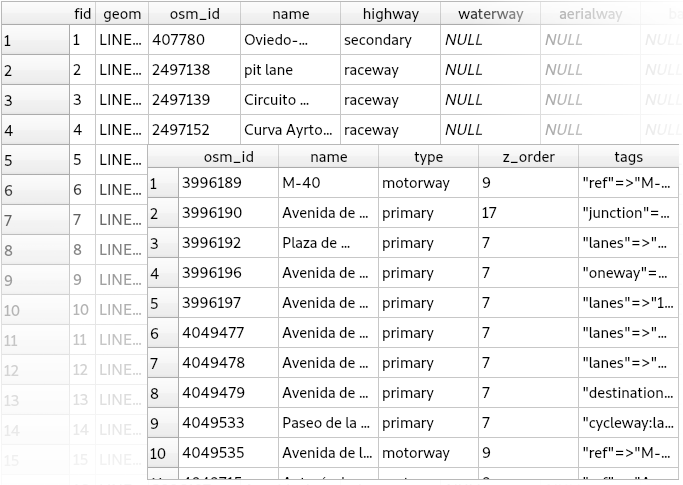
\includegraphics[width=.6\textwidth]{img/data_filtering.png}
		\caption[Filtrado por atributos específicos]{En este caso de filtrado por atributos, con datos en formato OpenStreetMap, se ha restringido aquellos posibles valores del campo \texttt{highway}, además de eliminado columnas no relevantes, obteniendo un conjunto de datos reducido pero más enfocado al análisis a desarrollar.}
	\end{figure}

	El realizar estas operaciones nos permite eliminar aquellos datos que no sean relevantes a lo que queremos analizar, minimizando el riesgo a error y la carga de procesamiento a realizar.

	\subsection*{Caso Práctico}
	Partiendo de los datos originales a nivel estatal, es decir, de toda España, se ha seleccionado solo aquellos datos que correspondían con carreteras aptas para vehículos motorizados (como coches) en el término municipal de Granada.
	Esto se ha realizado a través de las utilidades de \textit{Osmium}\footnote{Osmium: Proyecto con numerosas herramientas para trabajar con datos de OpenStreetMap. \url{https://osmcode.org/}}.
	
	\begin{minipage}{\textwidth}
	\textbf{\textit{Osmium Extract}} Se ha usado un polígono, descrito en \texttt{GeoJSON}, que corresponde al área municipal de Granada \autocite{GranadaPoly} y se ha invocado de la siguiente forma:
	
	\mint[autogobble,
	frame=single,
%	python3,
%	linenos,
	numbersep=6pt,
	fontsize=\scriptsize,
	bgcolor=mintedbg]{shell}{|>> osmium extract spain-latest.osm.pbf -p granada.json -o granada-latest.osm.pbf}
\end{minipage}

\begin{minipage}{\textwidth}
	\textbf{\textit{Osmium Tags Filter}} Se ha filtrado por todas las primitivas \textsc{Way} cuyo valor de \texttt{highway} comprenda las calles autorizadas para vehículos motorizados, de la siguiente manera:
	\mint[autogobble,
	frame=single,
%	python3,
%	linenos,
	breaklines,
	numbersep=6pt,
	fontsize=\scriptsize,
	bgcolor=mintedbg]{shell}{|>> osmium tags-filter granada-latest.osm.pbf 'w/highway=*_link' 'w/highway=motorway,trunk,primary,secondary,tertiary,residential,living_street' -o granada-latest-highways.osm.pbf}
\end{minipage}

\section{Estructura y Empaquetado}
	Como ya se ha explicado antes, \textit{GeoPackage} es en esencia un contenedor \textit{SQLite}, una base de datos relacional muy portable. Como tal, resulta un formato muy adecuado para datos compuestos por atributos, aunque no necesariamente estén relacionados entre sí.

	\begin{figure}[htbp]
		\centering
		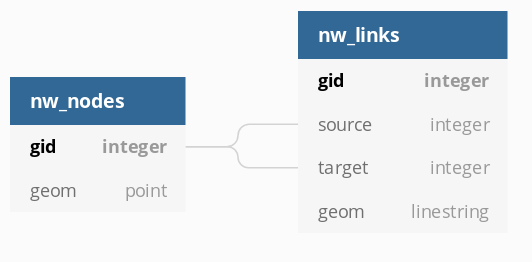
\includegraphics[width=.7\textwidth]{img/network_defn.png}
		\caption[Definición mínima de las entidades de una red]{Como mínimo, debe almacenarse la geometría, y un elemento identificativo, usado para referenciar los nodos en cada enlace, como nodos de origen y de objetivo.}
		\label{network_defn}
	\end{figure}

	Un \textit{GeoPackage} puede estar compuesto por entidades cualesquiera, pero en este caso concreto, necesitaremos dos entidades adicionales, una para nodos y otra para enlaces, tal y como se define en \autoref{network_defn}.
	
	A ambas entidades, como información interesante, se puede añadir una estimación de coste, bien en distancia o tiempo, restricciones de navegabilidad en una u otra dirección, entre otras. Esto se podría hacer directamente en la misma entidad, o en una entidad externa que contenga metadatos y referencie por el identificador
	
	\subsection*{Caso Práctico}
	En el caso práctico, se ha almacenado los datos de Granada, ya procesados y reducidos, sobre un fichero \textit{GeoPackage}. Esto se ha hecho gracias a una herramienta de \textit{GDAL}\footnote{\textit{GDAL/OGR}: Colección de herramientas de software libre para trabajar con datos geográficos. \url{https://gdal.org/}} llamada \textit{ogr2ogr}\footnote{\textit{ogr2ogr}: Herramienta para convertir entre formatos de datos geográficos.}.
	
	\mint[autogobble,
	frame=single,
	python3,
%	linenos,
	numbersep=6pt,
	fontsize=\scriptsize,
	bgcolor=mintedbg]{shell}{|>> osmium extract spain-latest.osm.pbf -p granada.json -o granada-latest.osm.pbf}
	
	Por razones prácticas, no creamos las entidades aún.Esto lo hacemos en el siguiente apartado, directamente con la herramienta que se ha desarrollado para generar la topología.
	
\section{Preparación de la Topología}
	Para generar una topología, tan solo necesitamos todas los enlaces que componen la red a analizar.
	Para crear una topología de dicha red, cada enlace ha de descomponerse en cada intersección entre dos o más enlaces. Para ello, aplicaremos un sencillo algoritmo definido en  \autoref{decompose_ways_algo}.
	
	\begin{listing}[htbp]
		\inputminted[autogobble,
			frame=single,
			python3,
%			linenos,
			numbersep=6pt,
			fontsize=\scriptsize,
			bgcolor=mintedbg,
		]{python}{algorithm_latex.py}
		\caption[Algoritmo para generar una topología]{Dado un conjunto de líneas, para cada línea, dividimos entre dos puntos intermedios, siempre y cuando estos sean válidos, hayan sido usado más de una vez en en el total de las líneas. Como invariante necesaria, se considera que tanto el primer y último punto de una línea son válidos.}
		\label{decompose_ways_algo}
	\end{listing}

	El objetivo de este proceso es la descomposición en unidades únicas, una por cada intersección encontrada a lo largo de una línea. Para llevar esto a cabo, debemos mantener un registro de cuántas veces se utiliza cada punto contenido en cada línea y subdividir cada línea entre dos nodos.
	Una vez tenemos la topología de red procesada, debemos almacenarla en el \textit{GeoPackage} conforme a la estructura descrita en \autoref{network_defn}.
	
	\begin{figure}[htbp]
		\begin{center}
	\begin{subfigure}{0.4\textwidth}
		\centering
		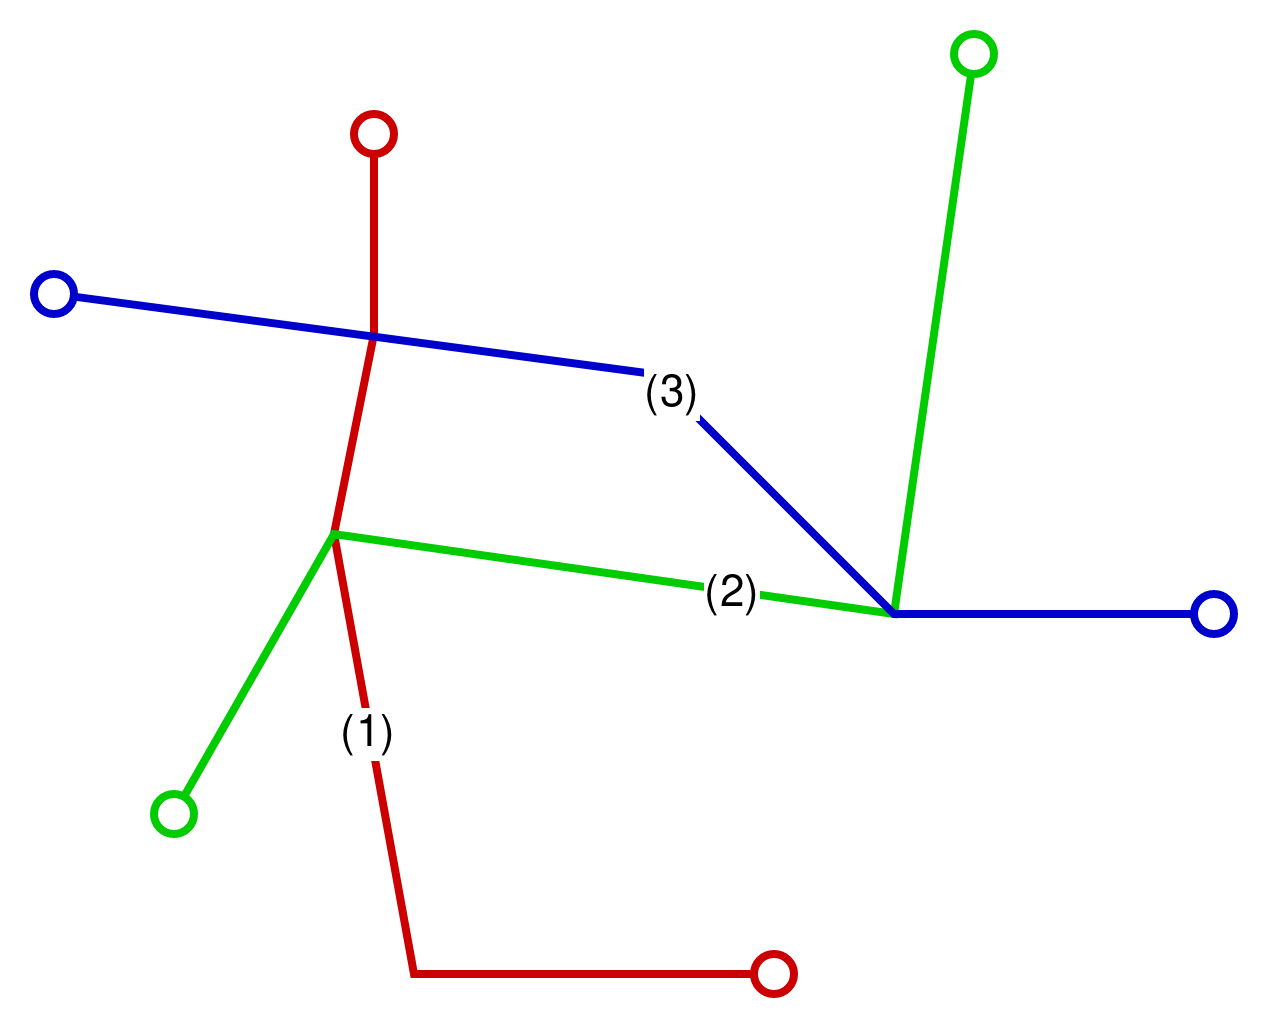
\includegraphics[width=.95\textwidth]{img/topology_before.png}
		\subcaption{Enlaces iniciales}
		\label{topology_before}
	\end{subfigure}
	\begin{subfigure}{0.4\textwidth}
		\centering
		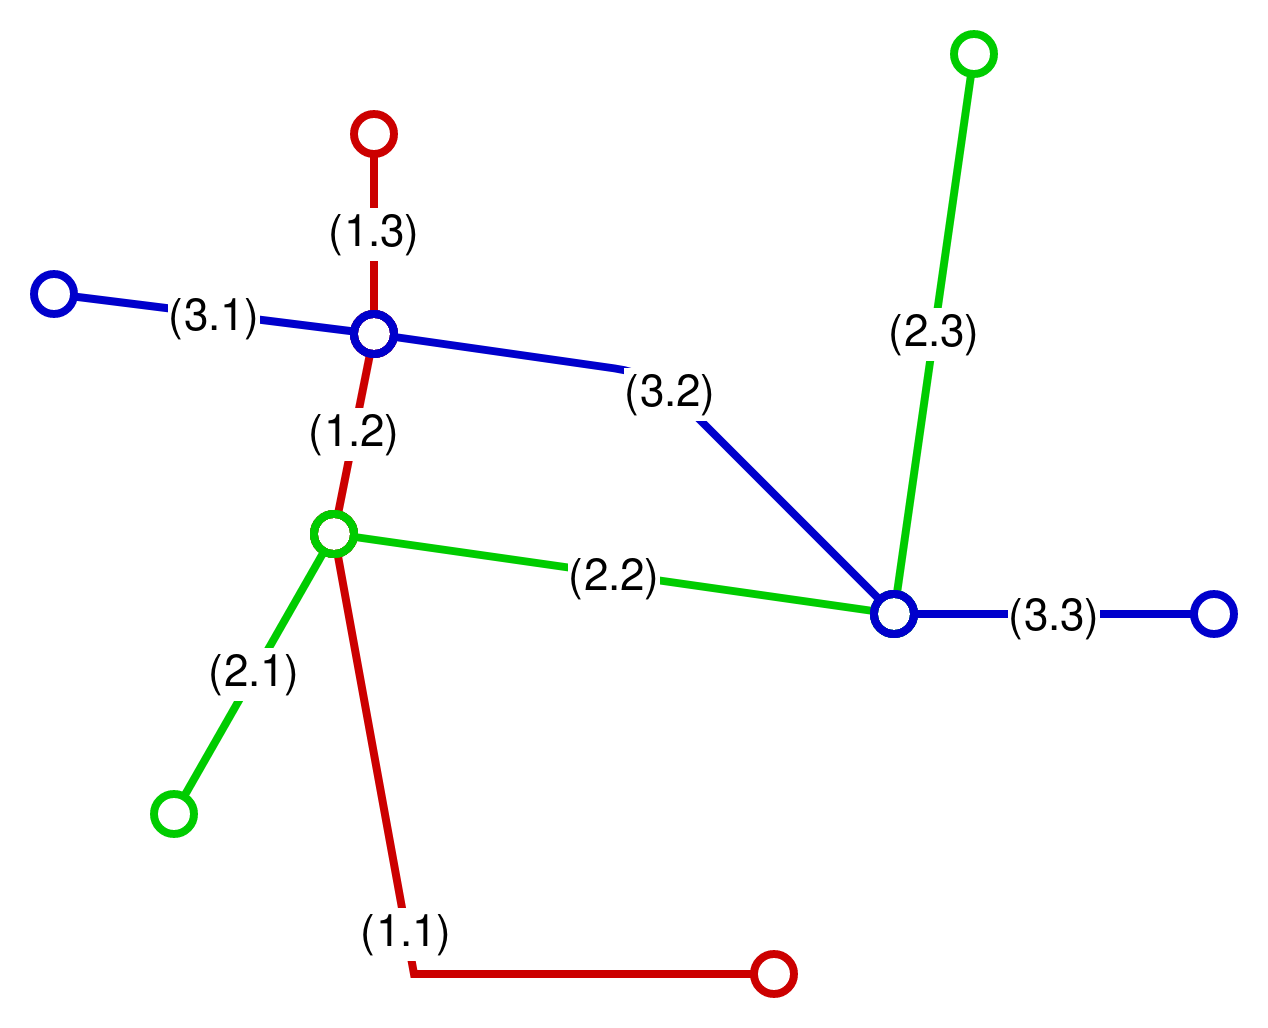
\includegraphics[width=.95\textwidth]{img/topology_after.png}
		\subcaption{Subenlaces resultantes}
		\label{topology_after}
	\end{subfigure}
\end{center}
	\caption[Descomposición topológica de una red]{Descomposición topológica de una red, nótese como cada intersección está delimitada con un redondel. Esto es porque cada enlace se ha dividido en varios enlaces, conservando los lados con varios puntos sin intersección en el proceso.}
	\end{figure}

	
	\subsection*{Caso Práctico}
	Para el caso práctico, se ha desarrollado un software \autocite{gpkgRouting}] en \textit{Python} que utiliza \textit{PyOsmium}\footnote{\textit{PyOsmium}: \textit{Bindings} en Python para la biblioteca \textit{Osmium}} para leer todos las primitivas \textsc{Way} de \textit{OpenStreetMap}. 
	
	\begin{listing}[htbp]
		\inputminted[autogobble,
		frame=single,
		python3,
%		linenos,
		breaklines,
		firstline=52,
		lastline=60,
		numbersep=6pt,
		fontsize=\scriptsize,
		bgcolor=mintedbg,
		]{python}{gpkgrouting/gpkgrouting/handlers.py}
		\caption[Carga de los datos de \textit{OpenStreetMap} con \texttt{gpkgRouting}]{El software carga todos las primitivas \textsc{Way} de un fichero OpenStreetMap y además, para cada elemento, realiza un conteo del número de usos de cada nodo.}
	\end{listing}
	
	Una vez hemos cargados todos los datos, se aplica el algoritmo descrito en \autoref{decompose_ways_algo} para descomponer los caminos en enlaces de una topología y posteriormente almacena la red en un \textit{DataFrame} de \textit{GeoPandas}\footnote{\textit{GeoPandas}: Extensión \textit{GIS} de \textit{Pandas}, \textit{framework} de \textit{Python} con estructuras \textit{DataFrame}, marcos de datos. \url{http://www.geopandas.org/}}, desde la cual exportaremos a GeoPackage. 
	Una vez realizado esto, se almacena el contenido del \textit{DataFrame} en el fichero \textit{GeoPackage} donde tenemos los datos de partida.
	
	\begin{listing}[htbp]
		\inputminted[autogobble,
		frame=single,
		python3,
%		linenos,
		breaklines,
		firstline=108,
		lastline=119,
		numbersep=6pt,
		fontsize=\scriptsize,
		bgcolor=mintedbg,
		]{python}{gpkgrouting/gpkgrouting/handlers.py}
		\caption[Definición de los datos finales obtenidos por \texttt{gpkgRouting}]{Los DataFrame de GeoPandas son una estupenda representación intermedia, ya que son contenedores muy eficientes y además gozan de mucha funcionalidad, como pueda ser directamente exportar a una base de datos \textit{GeoPackage}.}
	\end{listing}
		
	\begin{figure}[htbp]
		\centering
		\includegraphics[width=.9\textwidth]{img/granada_topology.png}
		\caption[Topología resultante, visualizada con el software \textit{QGIS}]{Resultado gráfico de la topología resultante al aplicar el software \texttt{gpkgRouting} y visualizado en \textit{QGIS}}
	\end{figure}

\section{Aplicación del Encaminamiento}
	En este momento, tenemos un \textit{GeoPackage} enrutable, el cual podemos inmediatamente utilizar o compartir con terceros como recurso. En el caso de aplicar inmediatamente alguna técnica de encaminamiento, debemos construir un grafo con la información almacenada en nuestro \textit{GeoPackage}.
	
	\begin{figure}[htbp]
		\centering
		\includegraphics[width=0.78\textwidth]{img/granada_shortest_path}
		\caption[Camino más corto (distancia) entre dos puntos]{Visualizamos el camino obtenido de \autoref{lst:qgis_gpkgrouting} en la suite \textit{QGIS}. En este caso, podemos ver que partimos de ETSIIT y acabamos cerca de la Cámara de Comercio de Granada.}
		\label{pathfinding_granada}
	\end{figure}
	
	Con el grafo ya construido, podremos aplicar algún algoritmo de búsqueda de caminos \autocite[255-287]{gvaliente} para el encaminamiento, existiendo mejores elecciones en función de los datos que tenemos. En el peor caso, siempre podremos aplicar un algoritmo en profundidad usando como coste la distancia de cada enlace.
	
	Heurísticas utilizables podrían ser también el tiempo medio que tarda un vehículo en recorrer una calle, si es que dispusiésemos de tal información. En el caso de haber subdividido un enlace, podríamos considerar la distancia de la división respecto a la distancia total y obtener de ahí un valor proporcional.
	
	\subsection*{Caso Práctico}
	A partir de \textit{NetworkX}\footnote{\textit{NetworkX}: \textit{Framework} de \textit{Python} para tratamiento y operaciones con grafos. \url{https://networkx.github.io/}}, se genera un grafo dirigido en el que todos los enlaces se representan como tuplas $(origen, destino)$ y tienen sus atributos concretos. Con el mismo, se aplican algoritmos como A* para calcular secuencias de nodos por los que pasar para encontrar el camino más óptimo.
	
	\begin{listing}[htbp]
		\begin{minted}[autogobble,
		frame=single,
		python3,
%		linenos,
		breaklines,
		numbersep=6pt,
		fontsize=\scriptsize,
		bgcolor=mintedbg,
		]{python}
		import geopandas as gpd
		import networkx as nx
		df = gpd.from_file('granada-latest-highways.gpkg', driver='GPKG', layer='nw_links')
		G = nx.from_pandas_edgelist(df, create_using=nx.DiGraph)
		
		try:
		path = nx.shortest_path(G, SOURCE, TARGET)
		# Do something with the retrieved path
		...
		except nx.NetworkXNoPath:
		# No path found
		...				
		\end{minted}
		\caption[Encaminamiento con \textit{GeoPackage} y \textit{NetworkX}]{\textit{Python} presenta un ecosistema muy maduro con multitud de herramientas, entre ellas \textit{GeoPandas} y \textit{NetworkX}, que nos permiten trabajar con datos \textit{GIS} y grafos de una forma indolora. Este último, además, tiene funcionalidades de búsqueda de caminos.}
	\end{listing}

\section{Conclusiones}
Dado el análisis y desarrollo llevado a cabo, cabe concluir que es posible almacenar topología en contenedores GeoPackage, y que estos pueden ser usados de forma reiterada para buscar caminos entre nodos de una red.

Es más, al ser un formato relativamente sencillo y casi universalmente aceptado, al ser una base de datos \textit{SQLite}, es trivial profundizar en ámbitos más específicos, que cubran casos de uso concretos. Lo inmediato, y muchas veces mencionado, sería su uso en terminales móviles que, sea por capacidades técnicas o software, no son capaces de aceptar otras soluciones para almacenamiento en local.

Esto, de igual forma, es complejo, ya que no existe un reglamento que enuncie cómo deben estructurarse los datos para que estos sean interpretados de una forma única y correcta, pero por suerte la especificación GeoPackage es abierta y extensible, permitiendo desarrollar extensiones para añadir funcionalidad\footnote{Véase un ejemplo esta extensión titulada \textit{Tiled Gridded Coverage Data Extension}.  \url{http://docs.opengeospatial.org/is/17-066r1/17-066r1.html}}.

Aún así, sea complejo o no, es una posibilidad más para empaquetar y compartir datos geográficos con la oportunidad de realizar consultas de encaminamiento, como herramientas como \textit{pgRouting}. Al fin y al cabo, un ingeniero debe conocer multitud de herramientas o tecnologías para decidir cual es la más conveniente para un problema concreto.